\subsubsection{Herstellung des Gehäuses}\label{hw_case_herstellung}
Zur Herstellung des Gehäuses kommt ein 3D-Drucker der Marke Creality 3D zum Einsatz. 
Der stark modifizierte Ender 3 Pro von Manuel Starz (vgl. Abb. \ref{fig:ender3}: \nameref{fig:ender3}) druckt die zuvor erstellten STL-Dateien mit PETG-Filament der Firma dasfilament. 
Der für den 3D-Druck nötige G-Code wird mit Ultimaker CURA generiert und mit Hilfe von OctoPrint (vgl. Abb. \ref{fig:octoprint}: \nameref{fig:octoprint}) an den Drucker übertragen. Das Gehäuse besteht aus vier Einzelteilen, je zwei Teile für die Seitenwände und zwei Teile für den Deckel.\par
\begin{figure}[H]
	\begin{center}
	\includegraphics[width=.5\textwidth]{img/ender3pro_mod.jpg}
	\end{center}
	\caption[3D-Drucker Ender 3 Pro (mod)]{3D-Drucker Ender 3 Pro (mod)}
	\label{fig:ender3}
\end{figure}
\begin{figure}[H]
	\includegraphics[width=1\textwidth]{img/gehäusedruck_octoprint_01.png}
	\caption[OctoPrint-Weboberfläche]{OctoPrint-Weboberfläche}
	\label{fig:octoprint}
\end{figure}
\noindent Die gedruckten Teile (vgl. Abb. \ref{fig:printet_parts}: \nameref{fig:printet_parts}) werden dann zum Teil mit Zwei-Komponenten-Epoxidkleber verbunden (vgl. Abb. \ref{fig:glued_parts}: \nameref{fig:glued_parts}) und mit Hilfe von Schleifpapier und einigen Schichten Klarlack zu einem klavierlackähnlichen Finish veredelt (vgl. Abb. \ref{filed_and_painted_parts}: \nameref{filed_and_painted_parts}). 
Die Seitenwände werden dann mit dem Bildschirm mit Hilfe des Zwei-Komponenten-Epoxidklebers und Heißkleber permanent verklebt (vgl. Abb. \ref{fig:finished_case_front}: \nameref{fig:finished_case_front}).
Danach wurden die Platinen und Kabel im Gehäuse angebracht (vgl. Abb. \ref{fig:finished_case_front}: \nameref{fig:finished_case_front}). 
Die Rückseite besteht der Einfachheit halber aus zwei identischen, punktsymmetrischen Teilen, die ebenfalls miteinander verklebt wurden.\par
\begin{figure}[H]
	\begin{subfigure}[b]{0.5\linewidth}
		\centering
		\includegraphics[width=1\textwidth]{img/druck_deckel.jpg}
		\caption[Druck eines der Deckel-Teile]{Druck eines der Deckel-Teile}
	\end{subfigure}
	\begin{subfigure}[b]{0.5\linewidth}
		\includegraphics[width=1\textwidth]{img/druck_waende.jpg}
		\caption[Druck der Wand-Teile]{Druck der Wand-Teile}
	\end{subfigure}
	\caption[Das Gehäuse entsteht]{Das Gehäuse entsteht}
	\label{fig:printing_parts}
\end{figure}
\par
\begin{figure}[H]
	\centering
	\begin{subfigure}[b]{0.3\linewidth}
		\includegraphics[width=1\linewidth]{img/gehauese_rueck.jpg}
		\caption[Rückseite]{Rückseite}
		\label{printet_parts_back}
	\end{subfigure}
	\begin{subfigure}[b]{0.3\linewidth}
		\includegraphics[width=1\linewidth]{img/gehauese_links.jpg}
		\caption[Linke Seite]{Linke Seite}
		\label{printet_parts_left}
	\end{subfigure}
	\begin{subfigure}[b]{0.3\linewidth}
		\includegraphics[width=1\linewidth]{img/gehauese_rechts.jpg}
		\caption[Rechte Seite]{Rechte Seite}
		\label{printet_parts_right}
	\end{subfigure}
	\caption[Ausgedruckte Teile des Gehäuses]{Ausgedruckte Teile des Gehäuses}
	\label{fig:printet_parts}
\end{figure}
\par
\begin{figure}[H]
	\begin{subfigure}[b]{0.5\linewidth}
		\centering
		\includegraphics[width=1\textwidth]{img/gehaeuse-verklebt.jpg}
		\caption[Verklebung des Gehäuses]{Verklebung des Gehäuses}
		\label{fig:glued_parts}
	\end{subfigure}
	\begin{subfigure}[b]{0.5\linewidth}
		\centering
		\includegraphics[width=1\textwidth]{img/gehaeuse-lakiert.jpg}
		\caption[Abgeschliffene und lackierte Teile]{Abgeschliffene und lackierte Teile}
		\label{fig:filed_and_painted_parts}
	\end{subfigure}
	\begin{subfigure}[b]{0.5\linewidth}
		\centering
		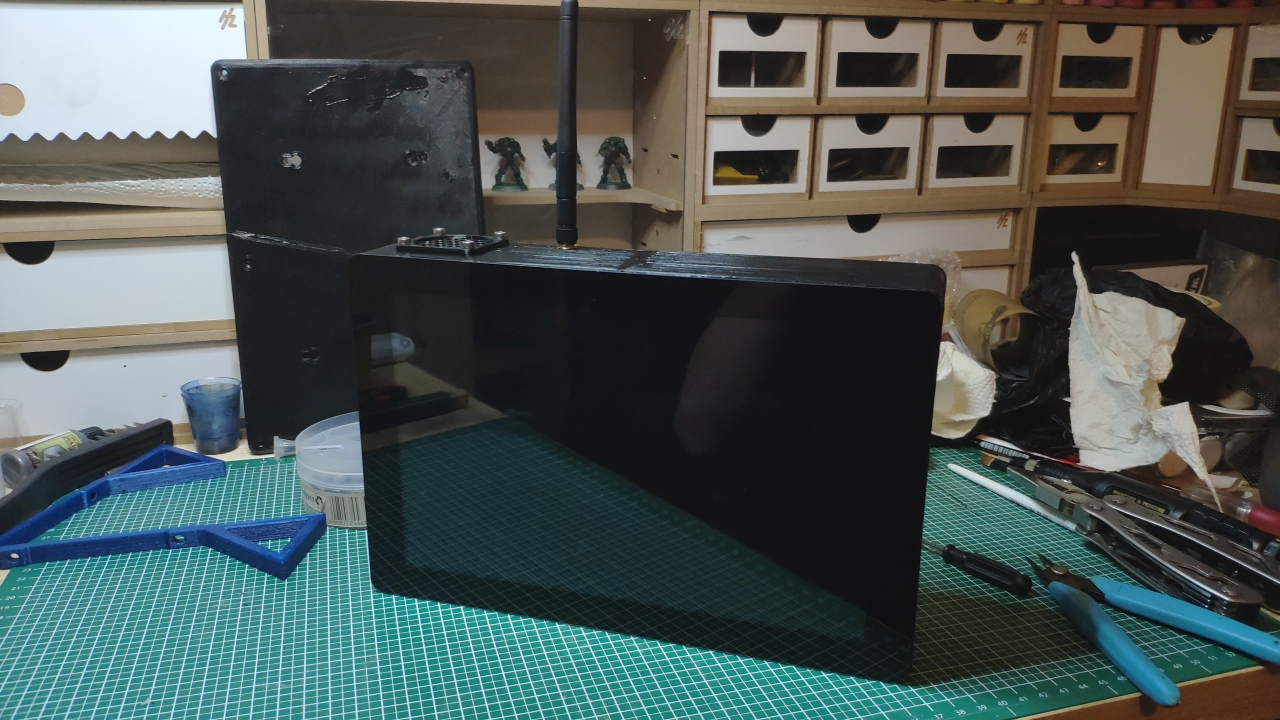
\includegraphics[width=1\textwidth]{img/geraet_front.jpg}
		\caption[Gehäuse und Bildschirm verklebt (von vorne)]{Gehäuse und Bildschirm verklebt (von vorne)}
		\label{fig:finished_case_front}
	\end{subfigure}
	\begin{subfigure}[b]{0.5\linewidth}
		\centering
		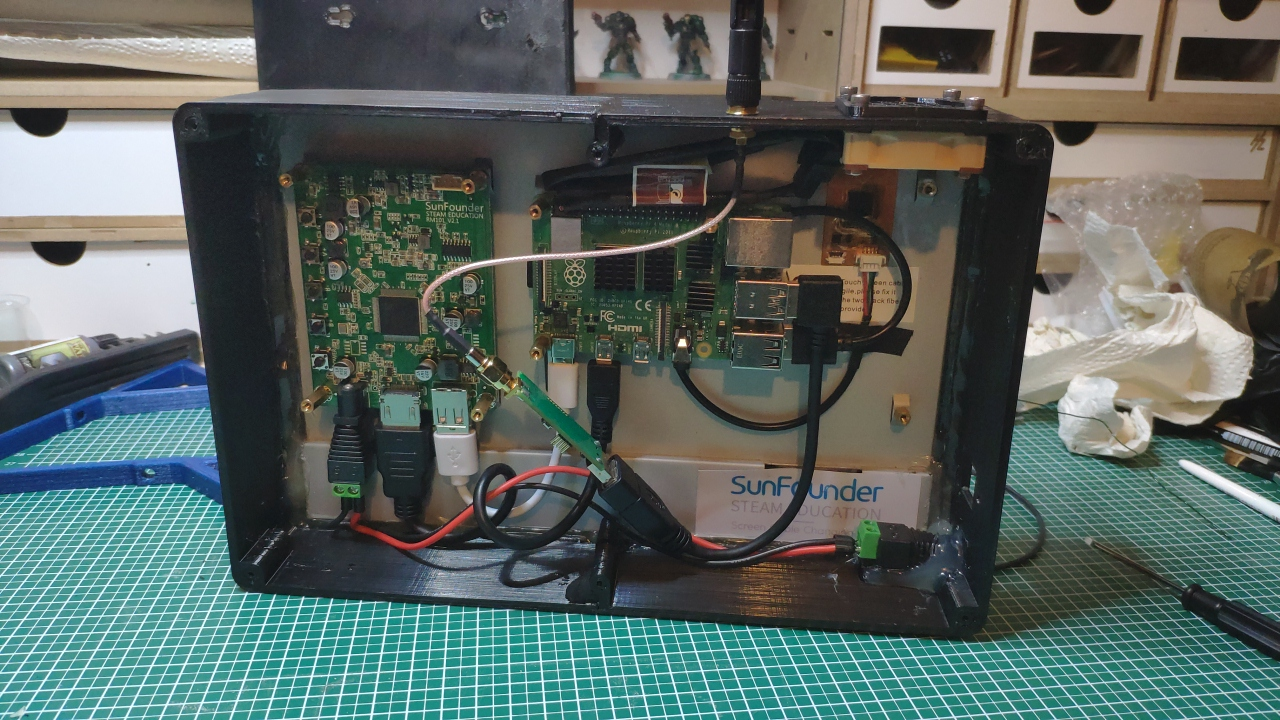
\includegraphics[width=1\textwidth]{img/geraet_rueck.jpg}
		\caption[Gehäuse und Bildschirm verklebt (von hinten)]{Gehäuse und Bildschirm verklebt (von hinten)}
		\label{fig:finished_case_back}
	\end{subfigure}
	\caption[Fertigung des Gehäuses]{Fertigung des Gehäuses}
	\label{fig:creating-case}
\end{figure}\par
\noindent Laut Ultimaker CURA beträgt die Gesamtdruckdauer des Gehäuses 36 Stunden 36 Minuten und verbraucht insgesamt 423 Gramm des verwendeten Filaments (dasFilament PETG Schwarz). 
Damit belaufen sich die Materialkosten des Gehäuses auf 11,61\euro{}\footnote{Genauere Kostenrechnung siehe Abschnitt \ref{ku_kosten_druck}: \nameref{ku_kosten_druck}}.\par
\noindent Bei der Herstellung ist es aber zu einem Problem gekommen. 
Die Stützstrukturen haben den Druck am Lüftereinlass gestört, was dazu führt, dass das Lüftergitter an der  linken Seitenwand (vgl. Abb. \ref{printet_parts_left}: \nameref{printet_parts_left}) nicht richtig gedruckt wurde und die losen Filamentstücke zu Macken an den Gehäusewänden führen.